\chapter{Inclusive CLFV Signals}
\label{chap:Signal}

As discussed in \autoref{chap:History}, the \ac{CLFV} processes involving top quarks have been studied by the \ac{ATLAS} and \ac{CMS} Collaborations in many orthogonal channels. Among all possible charged-lepton flavor mixing modes (i.e. e$\upmu$, e$\uptau$, and $\upmu\uptau$), the e$\upmu$ mode receives the most extensive scrutiny~\cite{ATLAS-CONF-2018-044,CMS:2022ztx,CMS:2023phe}, yielding a very tight constraint at $\mathcal{O}(10^{-8})$ on $\mathcal{B}(\tto{q})$. On the other hand, there exists only one preliminary study on the $\upmu\uptau$ mode carried out by the \ac{ATLAS} Collaboration~\cite{ATLAS-CONF-2023-001}, and the e$\uptau$ mode remains completely unexplored at the \ac{LHC} experiments. Therefore, the objective of this analysis is to probe as many unexplored channels as possible and search for all three charged-lepton flavor mixing modes simultaneously using data collected by the \ac{CMS} detector in 2016-2018. \autoref{sec:Target} gives a brief description of the targeted final states while signal event generation is described in \autoref{sec:SigGen}.
%%%%%%%%%%%%%%%%%%%%%%%%%%%%%%%%%%%%%%%%%%%
%%%%%%%%%%%%%%%%%%%%%%%%%%%%%%%%%%%%%%%%%%%
\section{Targeted Final States}
\label{sec:Target}

One of the central features of this analysis is the inclusion of a hadronic tau lepton, which remains relatively unexplored in the top quark sector. The target final states of this analysis contain exactly two light leptons (electron or muon) and one hadronic tau. The two light leptons can come with any flavor and charge compositions, as long as the sum of the electric charges of all three leptons is 1 or -1. Effectively, this guarantees all three lepton flavor mixing modes are covered by this analysis. In addition to leptons, the target final states at \ac{LO} also feature one or two jets with exactly one jet originating from a b quark and some imbalances in $\pt$ caused by neutrinos. Representative Feynman diagrams are shown in Figure~\ref{fig:Target}.

 \begin{figure}[tbh!]
 \begin{center}
 \begin{tabular}{ccc}
 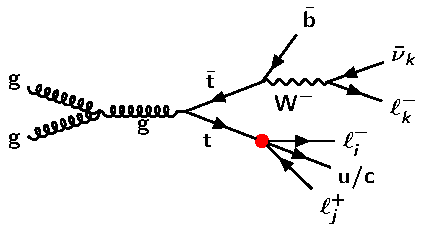
\includegraphics[width=0.33\textwidth]{figures/Part4/Signal/TT}&
 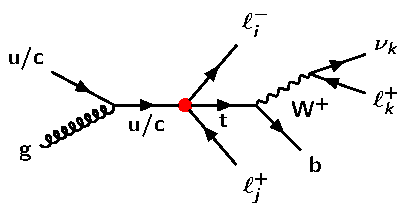
\includegraphics[width=0.33\textwidth]{figures/Part4/Signal/ST1}&
 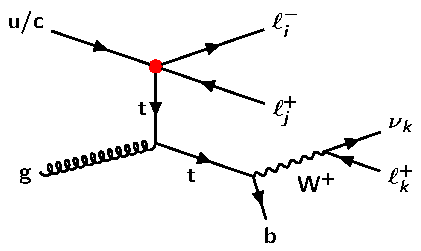
\includegraphics[width=0.33\textwidth]{figures/Part4/Signal/ST2}\\
 \end{tabular}
 \caption{Representative Feynman diagrams for the signal processes that are targeted by this analysis. Both top quark decay (left) and production (middle and right) \ac{CLFV} processes are shown. The indices $i$, $j$, and $k$ are lepton-flavor indices that run from 1 to 3 with the following conditions: i) $i\neq j$, ii) one of these three indices is 3, and iii) the other two are smaller than 3.}
 \label{fig:Target}
 \end{center}
 \end{figure}

Even though the e$\upmu$ flavor mixing mode is covered by this analysis, the corresponding processes can only enter the event selection through the \ac{OS}-e$\upmu$ channel with a hadronic tau produced by the \ac{SM} top quark. Depending on the charge assignment, the same event topology may also contribute to the e$\uptau$ or $\upmu\uptau$ modes, as the hadronic tau may also come from the flavor-violating vertex. Furthermore, the e$\uptau$ and $\upmu\uptau$ signals can enter the event selection through \ac{SS} dilepton channels, where the background yields are much lower. Therefore, it is expected that this analysis is more competitive in its sensitivity on e$\uptau$ and $\upmu\uptau$ modes.
%%%%%%%%%%%%%%%%%%%%%%%%%%%%%%%%%%%%%%%%%%%
%%%%%%%%%%%%%%%%%%%%%%%%%%%%%%%%%%%%%%%%%%%
\section{Signal Event Generation}
\label{sec:SigGen}

In general, the strategy to generate the \ac{CLFV} signal events for this analysis is very similar to the existing strategy described in \autoref{sec:Signals}. One notable distinction is that all three charged-lepton flavor mixing modes are enabled in samples produced for this analysis. This is achieved by explicitly turning on the e$\uptau$ and $\upmu\uptau$ terms in the \ac{EFT} operators. For example, the parameterization of the scalar-like operator specified in Equation~(\ref{eq:1:4}) is modified as,

\begin{eqnarray}
\textsf{C}_{\textsf{lequ}}^{(1)}  
 &=& \textsf{C}_{\textsf{lequ}}^{(1)1213}
 + \textsf{C}_{\textsf{lequ}}^{(1)2113}
 + \textsf{C}_{\textsf{lequ}}^{(1)1231}
 + \textsf{C}_{\textsf{lequ}}^{(1)2131} \nonumber\\
 &+& \textsf{C}_{\textsf{lequ}}^{(1)1313}
 + \textsf{C}_{\textsf{lequ}}^{(1)3113}
 + \textsf{C}_{\textsf{lequ}}^{(1)1331}
 + \textsf{C}_{\textsf{lequ}}^{(1)3131} \\
 &+& \textsf{C}_{\textsf{lequ}}^{(1)2313}
 + \textsf{C}_{\textsf{lequ}}^{(1)3213}
 + \textsf{C}_{\textsf{lequ}}^{(1)2331}
 + \textsf{C}_{\textsf{lequ}}^{(1)3231}. \nonumber
\label{eq:example}
\end{eqnarray}

This is only done to simplify the \ac{MC} production procedure as the number of unique samples can be reduced by a factor of three. From a theoretical point of view, each flavor mixing mode corresponds to an independent \ac{WC} without any presumed correlations with other \acp{WC}. The generated signal events from one sample are therefore categorized into three groups using information at the generator level. Since the lepton masses are neglected in the \ac{ME} calculation, the theoretical cross-section is identical across different flavor mixing modes. Therefore, events from all three groups are normalized to the same cross-section listed in Table~\ref{tab:signal}. 

The effective Lagrangian is implemented using the SMEFTsim~\cite{Brivio:2017btx} model, which is the common standard agreed by corresponding physics working groups of the \ac{ATLAS} and \ac{CMS} Collaborations. Other than the differences in signal cross-sections reported by different models, the \ac{CKM} and \ac{PMNS} matrices are also treated differently by SmeftFR~\cite{Dedes:2019uzs} and SMEFTsim. More specifically, nonzero off-diagonal terms are added to the entries of the \ac{CKM} and \ac{PMNS} matrices by SmeftFR while both matrices are set to identity by SMEFTsim. Effectively, this means SMEFTsim allows no contributions from \acp{FCCC} to the signal processes. Consequently, this results in a softer kinematic distribution of final-state particles even though the difference is largely negligible, as is shown in Figure~\ref{fig:reweight}.

Leptons that emerge from the \ac{EFT} vertex are generally far more energetic in the top quark production events than the top quark decay events. This notable distinction between the two signal modes is exploited to benefit sensitivity, which is discussed in \autoref{sec:SRInclusive}. Representative kinematic distributions of the simulated signal events at the generator level are shown in Figure~\ref{fig:SigGen}.

 \begin{figure}[tbh!]
 \begin{center}
 \begin{tabular}{ccc}
 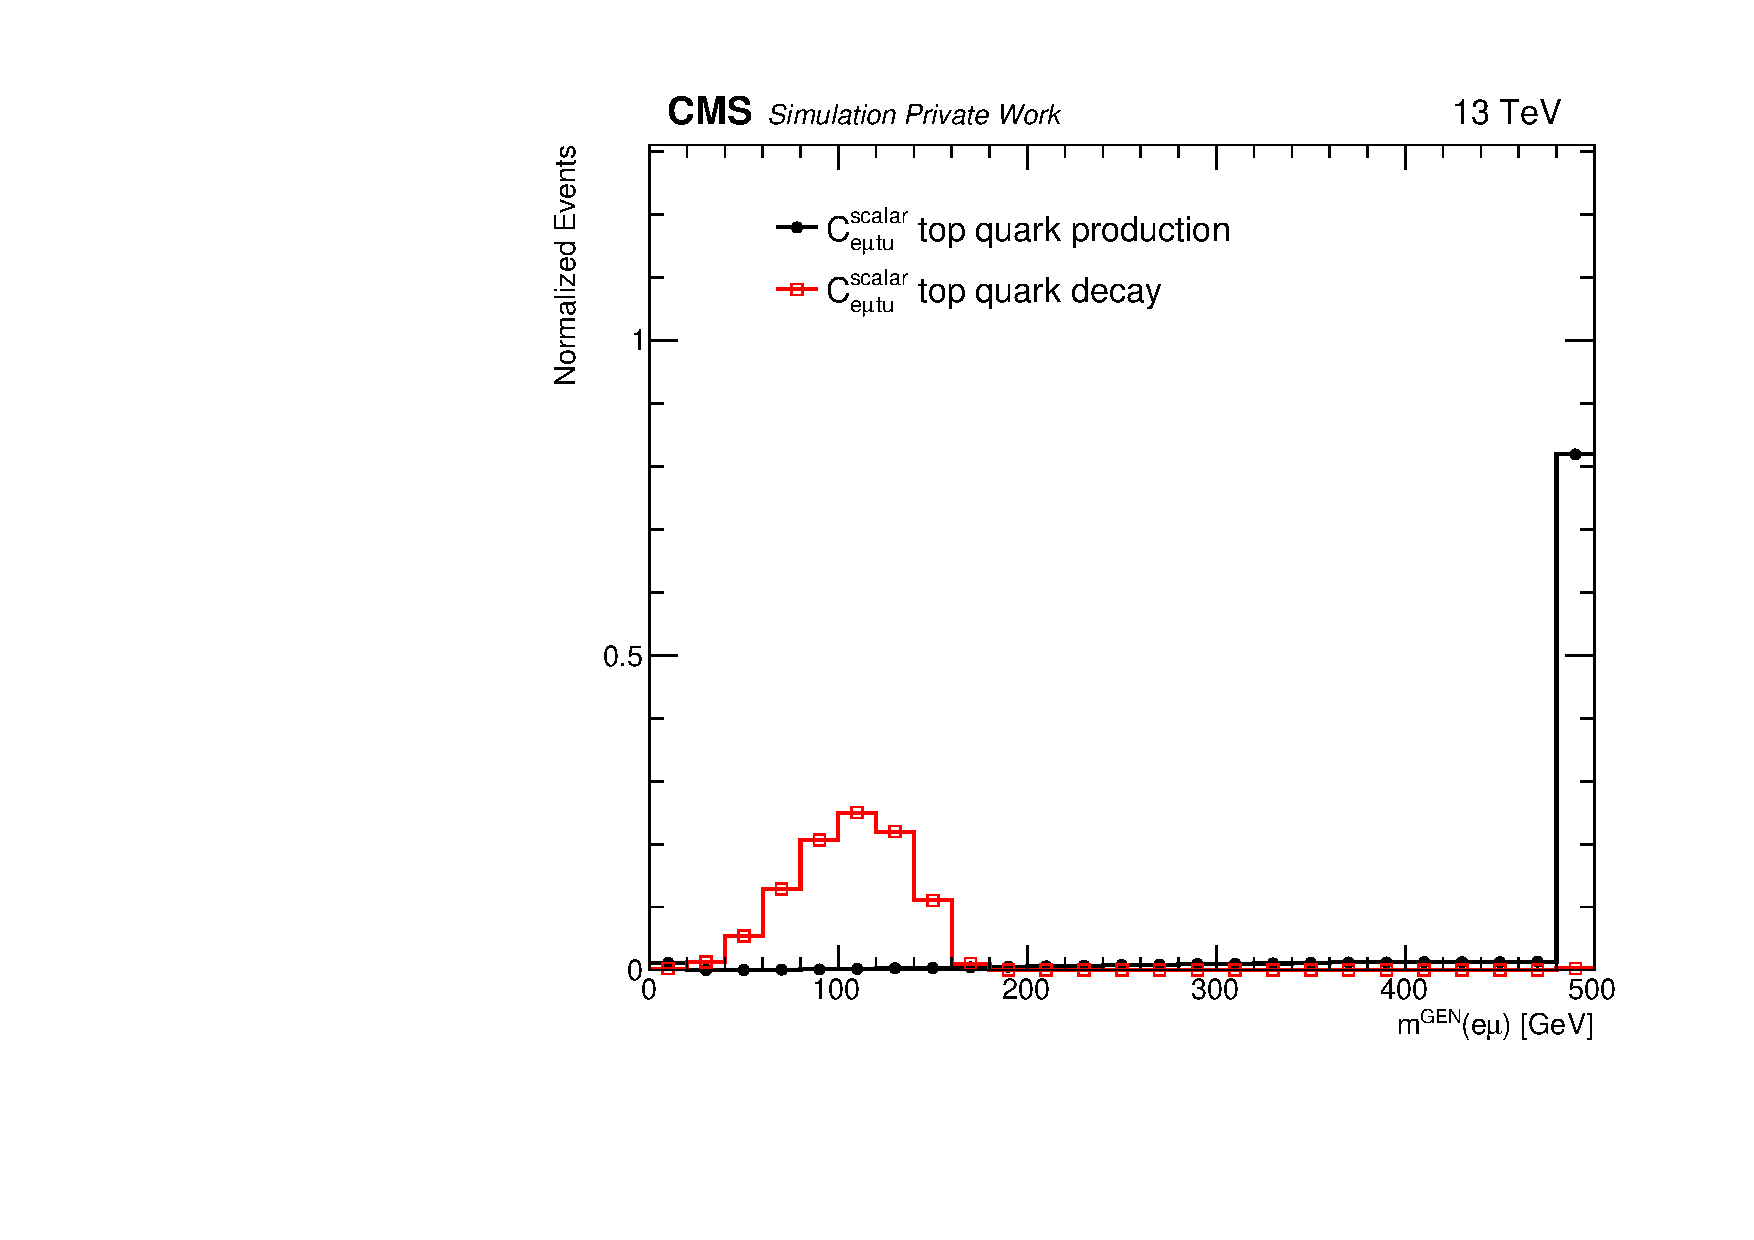
\includegraphics[width=0.33\textwidth]{figures/Part4/Signal/llM_emu}&
 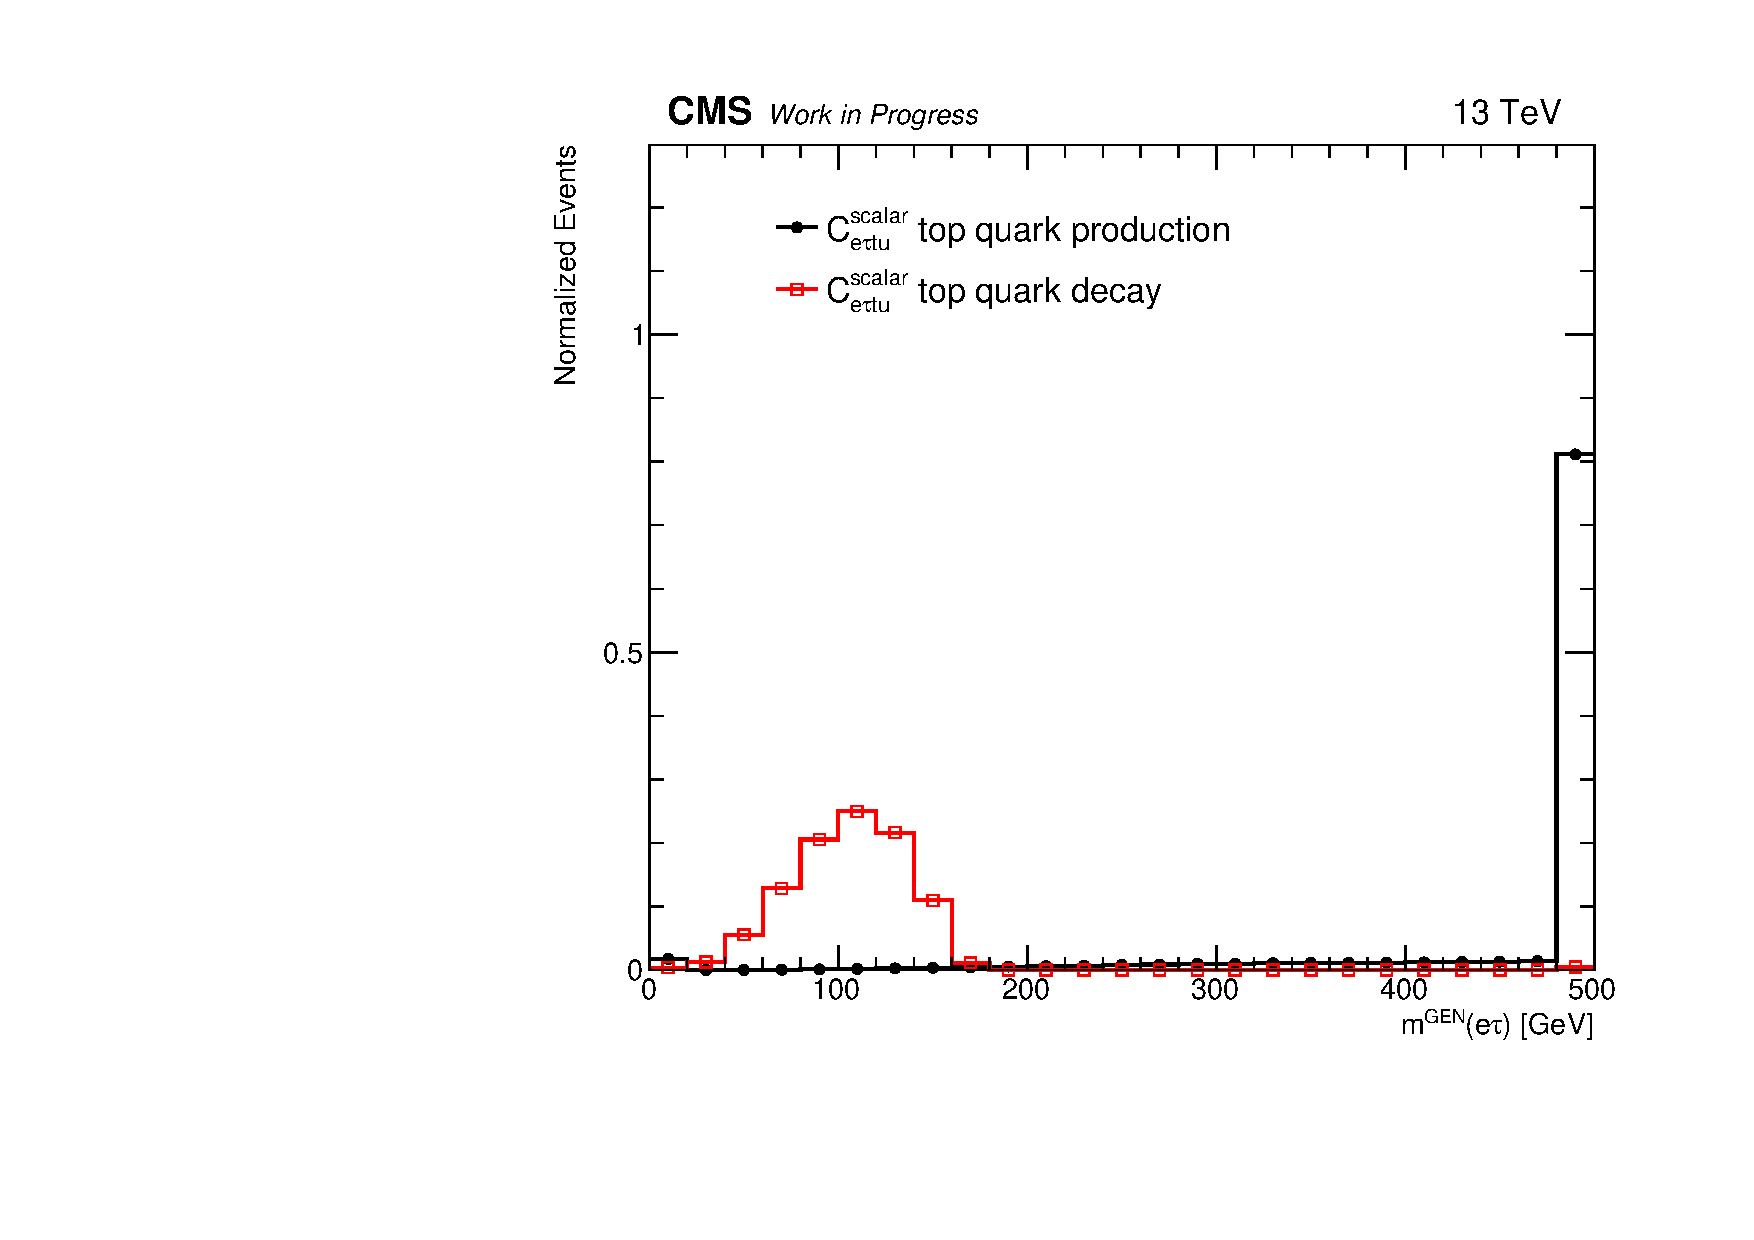
\includegraphics[width=0.33\textwidth]{figures/Part4/Signal/llM_etau}&
 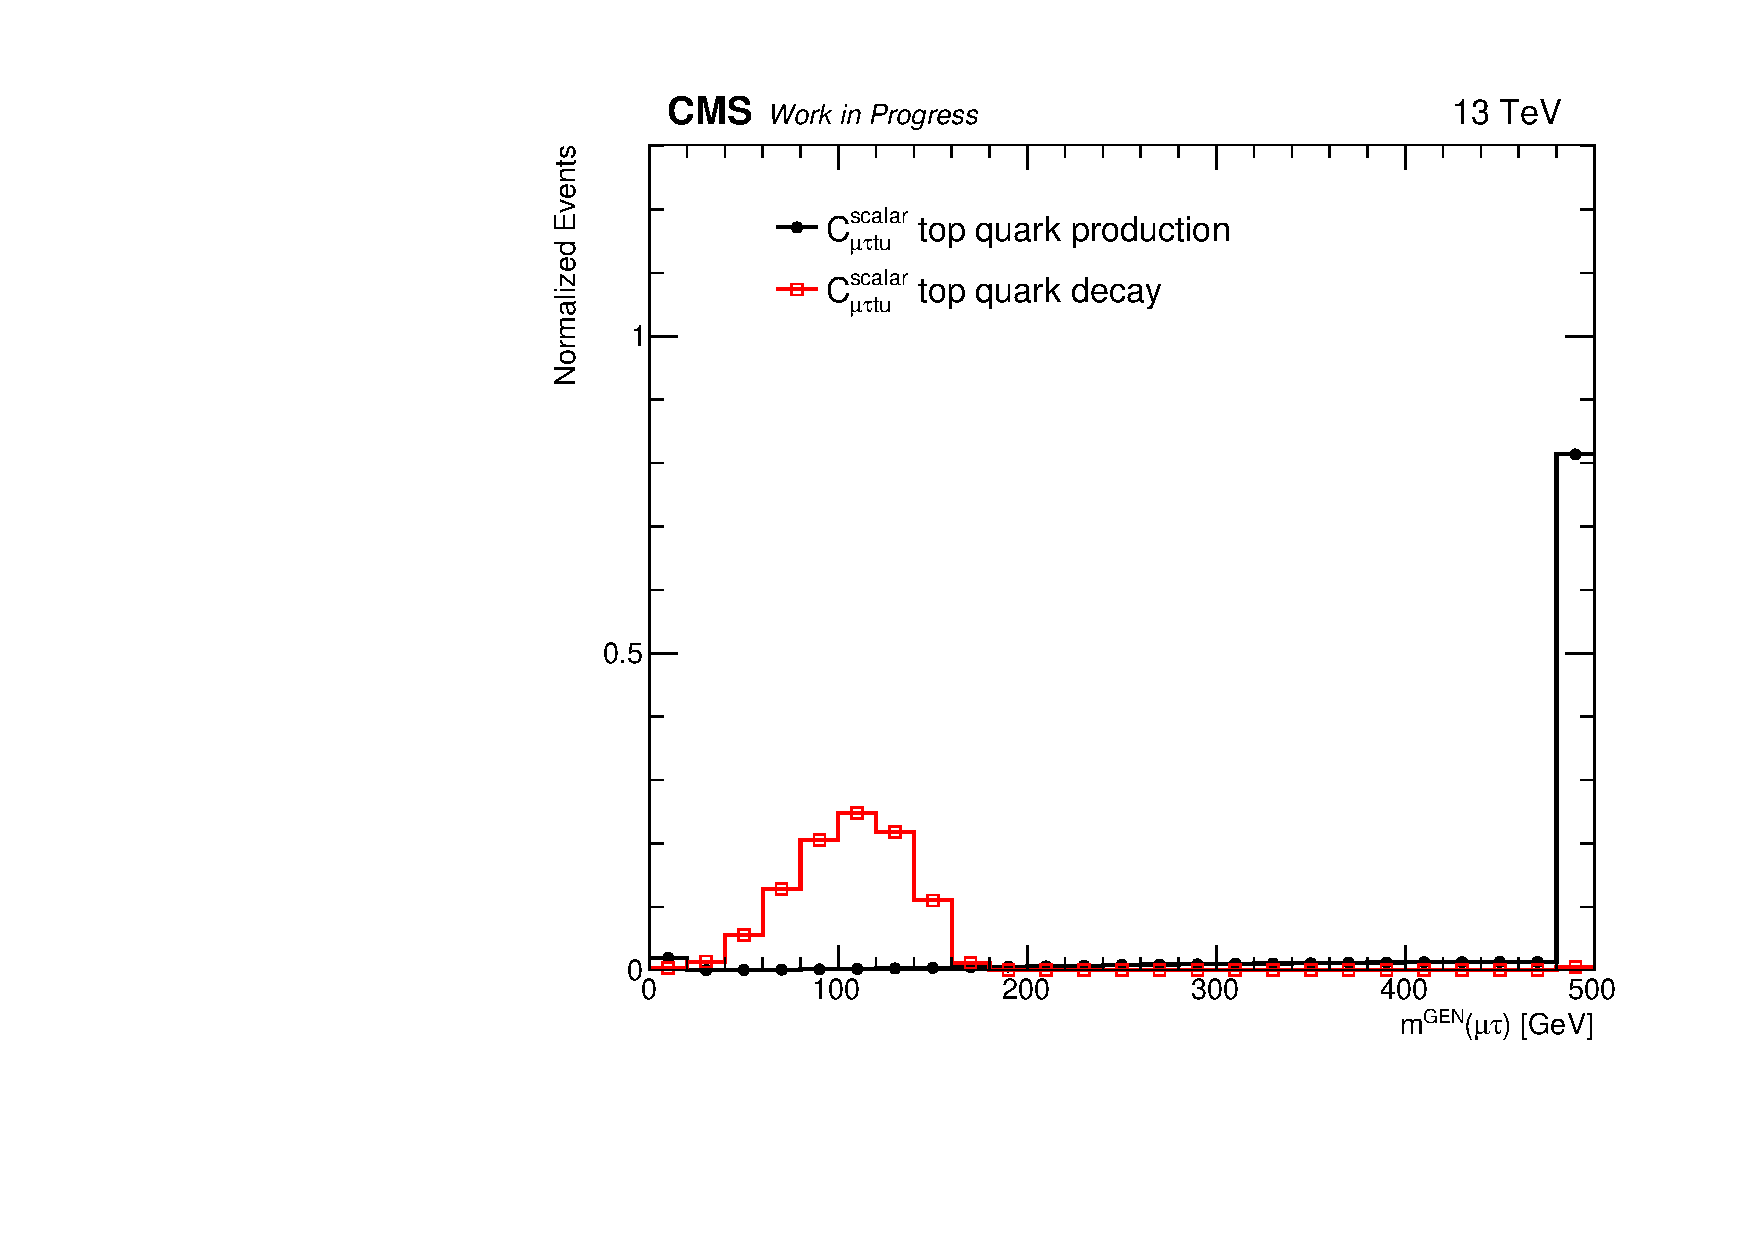
\includegraphics[width=0.33\textwidth]{figures/Part4/Signal/llM_mutau}\\
 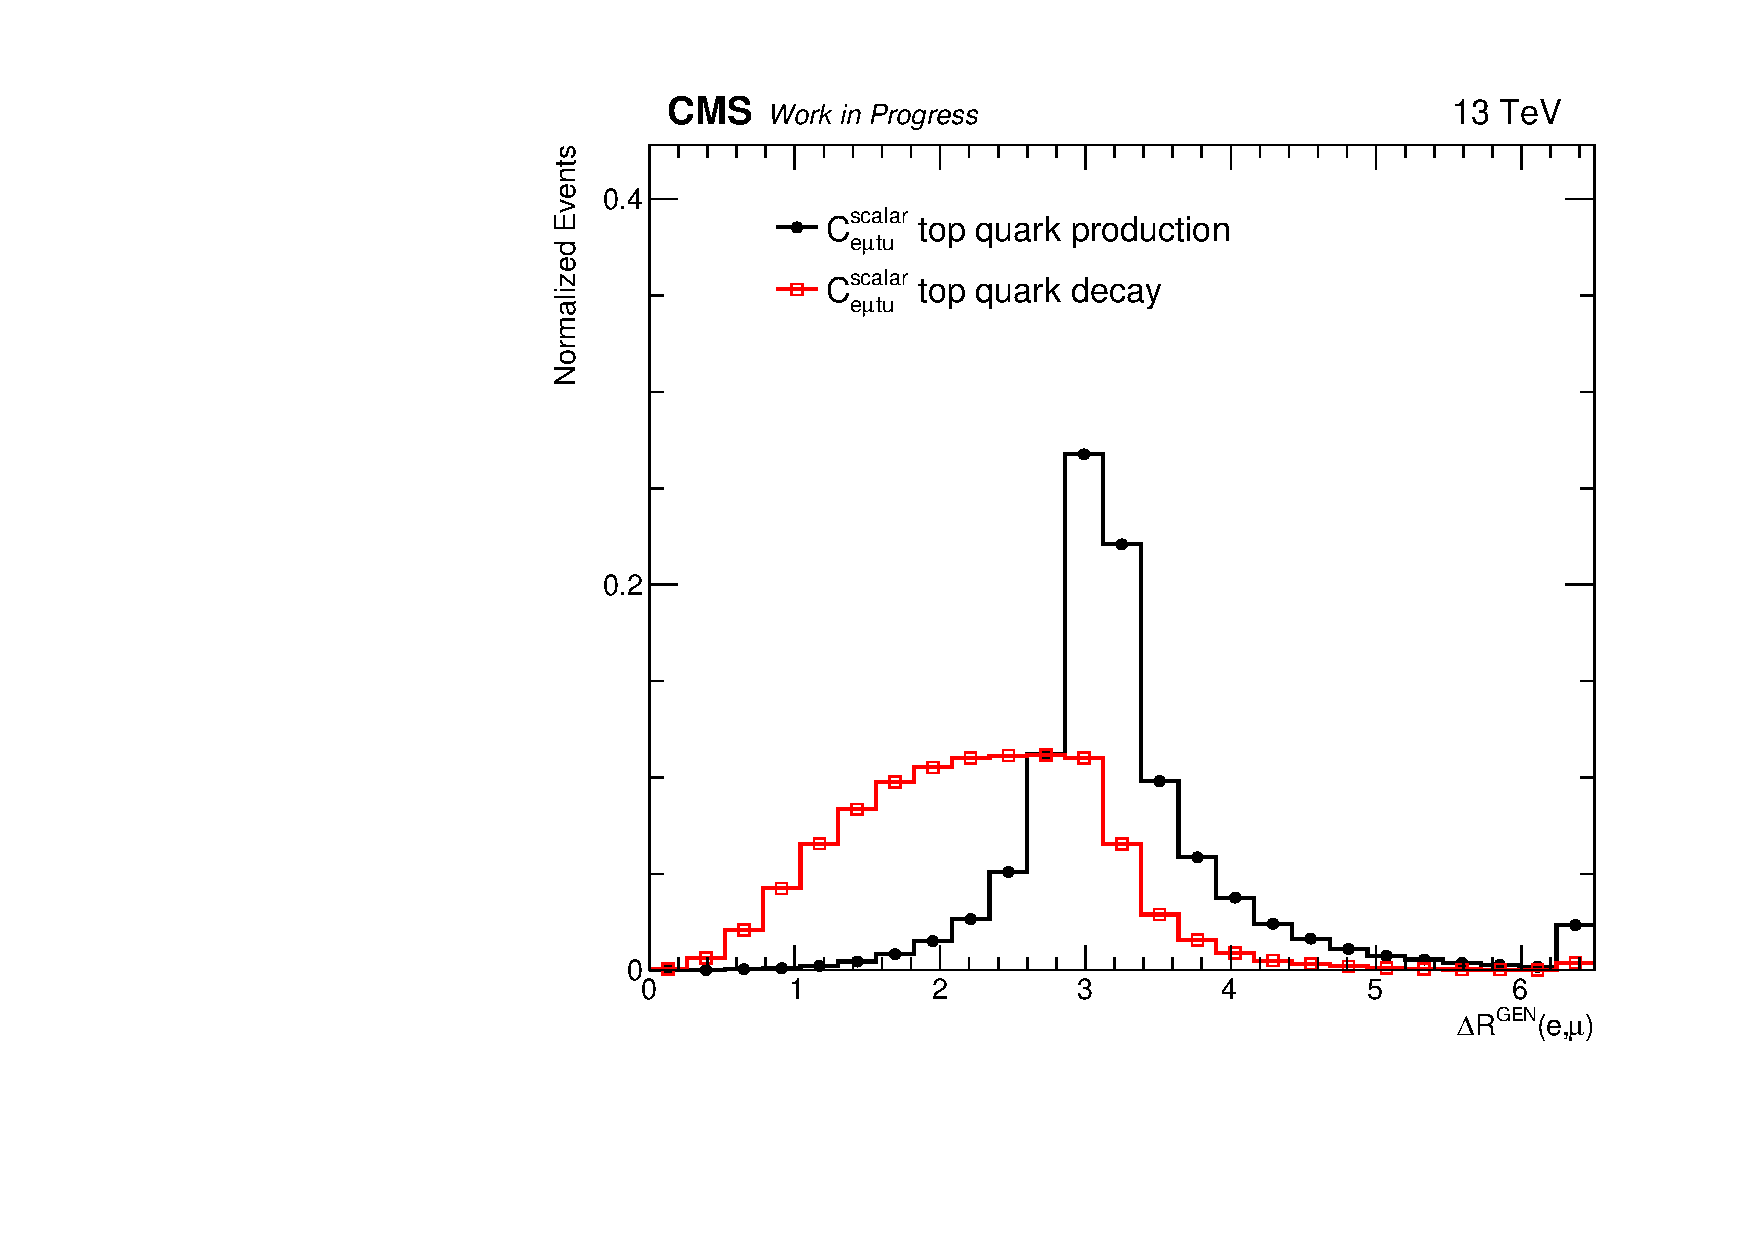
\includegraphics[width=0.33\textwidth]{figures/Part4/Signal/llDr_emu}&
 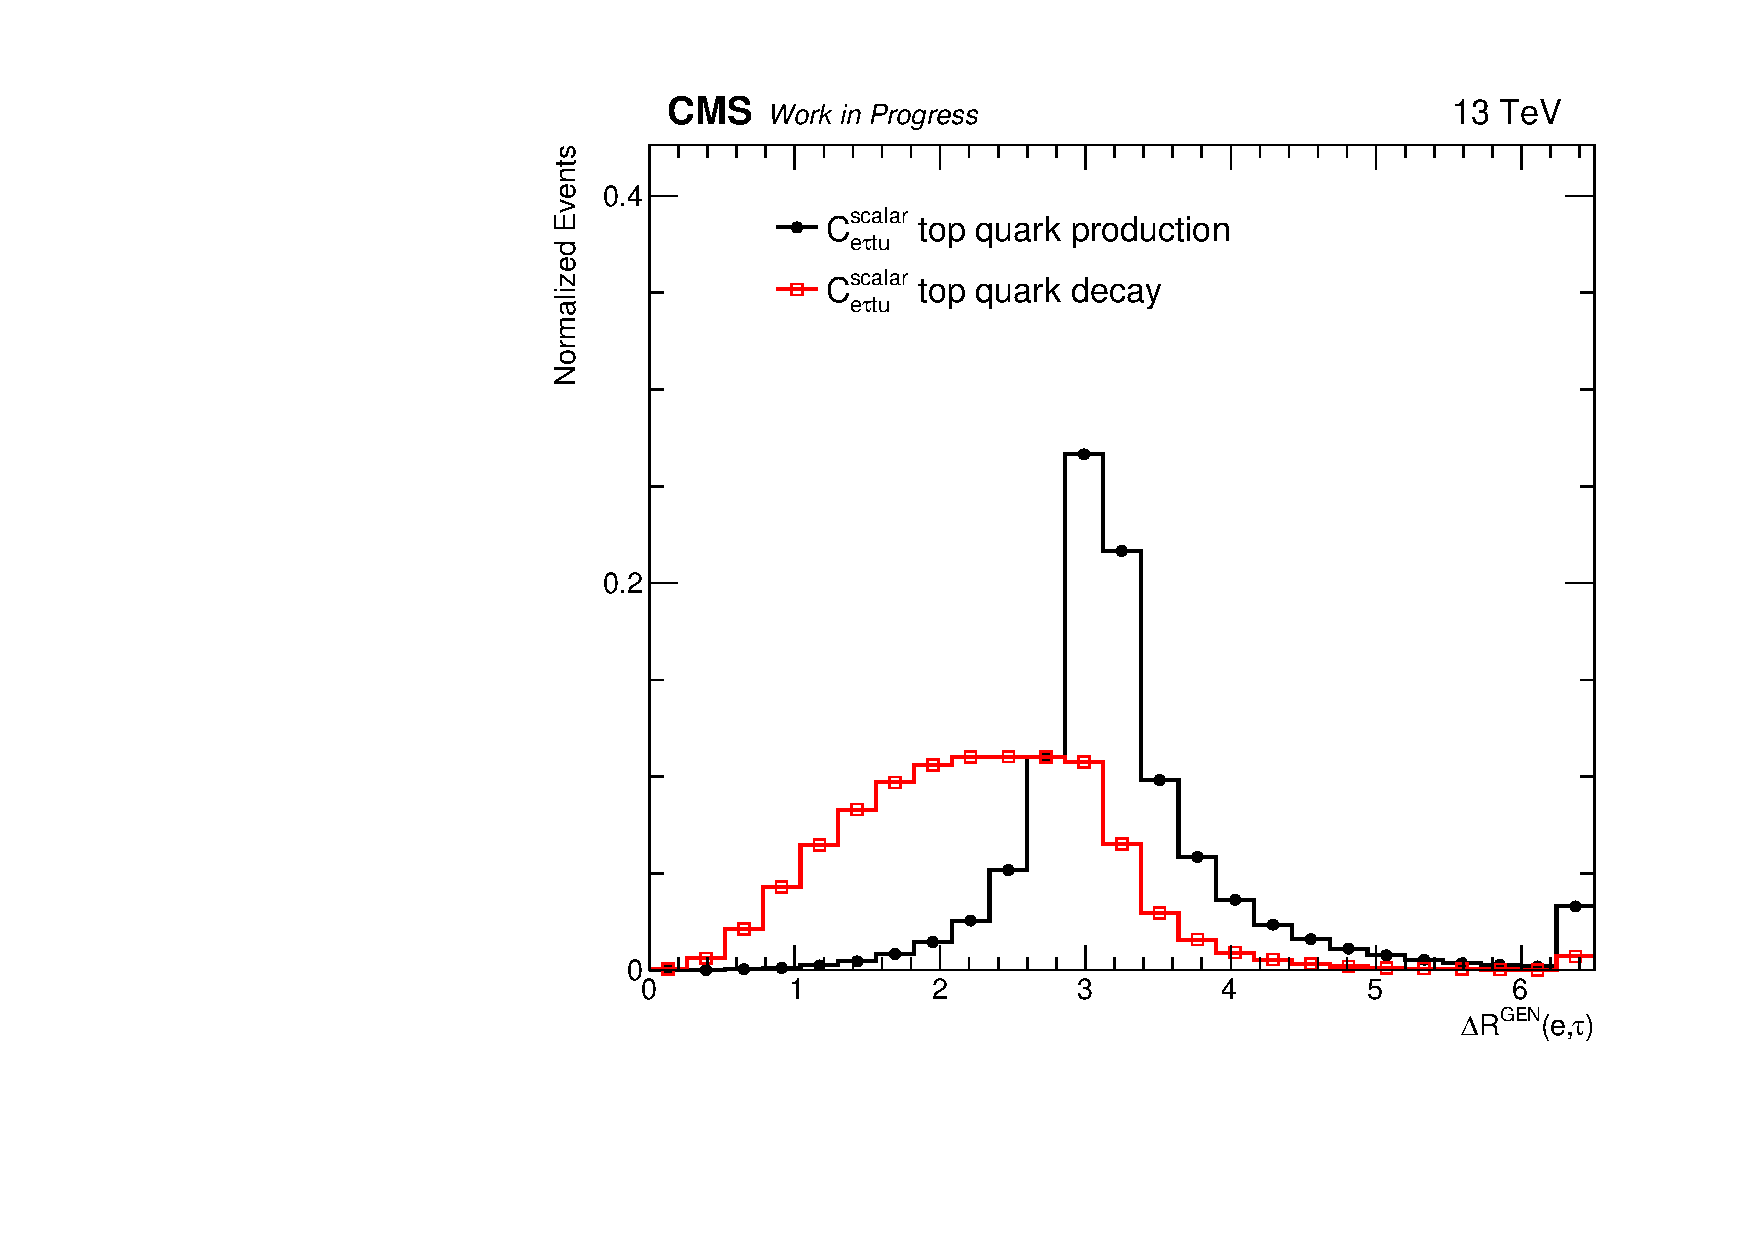
\includegraphics[width=0.33\textwidth]{figures/Part4/Signal/llDr_etau}&
 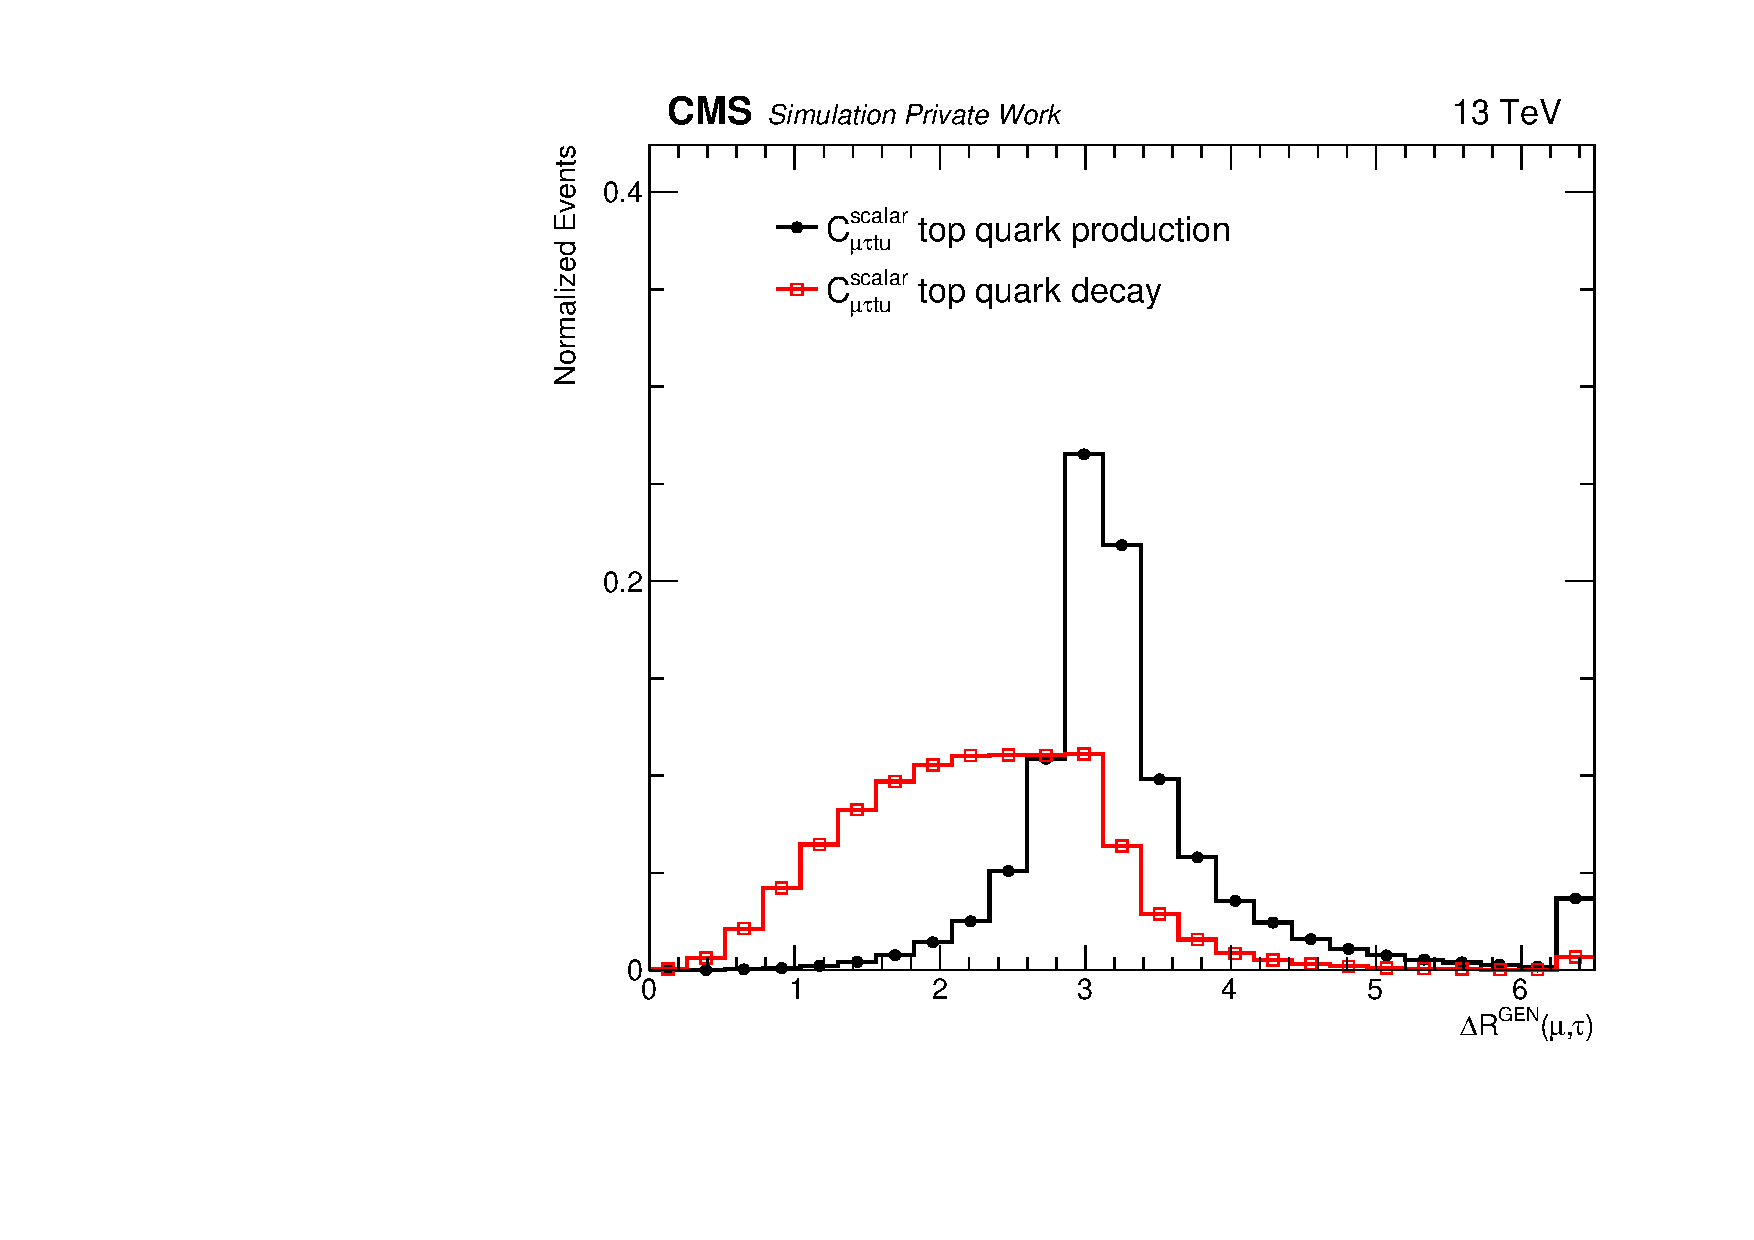
\includegraphics[width=0.33\textwidth]{figures/Part4/Signal/llDr_mutau}\\
 \end{tabular}
 \caption{Normalized kinematic distributions of the \ac{CLFV} signal events at the generator level. These events are generated by the scalar-like operator involving an up quark in the \ac{EFT} vertex. Events from the original samples are categorized into the e$\upmu$ (left), e$\uptau$ (middle), and $\upmu\uptau$ (right) modes. Distributions of the LFV dilepton mass and the opening angle between the two LFV leptons are shown in the top row and the bottom row, respectively. The top quark decay signals are shown in a red line with an open square while the top quark production signals are shown in a black line with a closed circle.}
 \label{fig:SigGen}
 \end{center}
 \end{figure}